\documentclass[11pt,letterpaper]{article}
\usepackage{amssymb,amsfonts,color,graphicx,amsmath,enumerate}
\usepackage{tikz}
\usepackage{amsthm,hyperref}

\newcommand{\naturals}{\mathbb{N}}
\newcommand{\integers}{\mathbb{Z}}
\newcommand{\complex}{\mathbb{C}}
\newcommand{\reals}{\mathbb{R}}
\newcommand{\exreals}{\overline{\mathbb{R}}}
\newcommand{\mcal}[1]{\mathcal{#1}}
\newcommand{\mable}{measurable}
\newcommand{\quats}{\mathbb{H}}
\newcommand{\rationals}{\mathbb{Q}}
\newcommand{\norm}{\trianglelefteq}
\newcommand{\Aut}{\text{Aut}}
\newcommand{\disk}{\mathbb{D}}
\newcommand{\halfplane}{\mathbb{H}}
\newcommand{\Lp}[2]{\left\|{#1}\right\|_{L^{#2}}}
\newcommand{\supp}[1]{\text{supp}({#1})}
\newcommand{\Hom}[2]{\text{Hom}_{{#1}}({#2})}
\newcommand{\tr}{\text{tr}}
\newcommand{\field}[1]{\mathbb{F}_{{#1}}}
\newcommand{\Gal}[1]{\text{Gal}\left({#1}\right)}
\newcommand{\esssup}{\text{ess sup }}
\newcommand{\essinf}{\text{ess inf }}
\newcommand{\affine}{\mathbb{A}}
\newcommand{\E}{\mathbb{E}}
\newcommand{\Prob}{\mathbb{P}}

\newenvironment{solution}
{\begin{proof}[Solution]}
{\end{proof}}

\theoremstyle{plain}
\newtheorem{theorem}{Theorem}

\theoremstyle{definition}
\newtheorem{definition}{Definition}
\newtheorem{example}{Example}

\voffset=-3cm
\hoffset=-2.25cm
\textheight=24cm
\textwidth=17.25cm
\addtolength{\jot}{8pt}
\linespread{1.3}

\begin{document}
%\noindent{\em Liam Hardiman\hfill{Date} }
\begin{center}
{\bf \Large Week 1 - Entropy (Speaker: Roman Vershynin)}
\vspace{0.2cm}
\hrule
\end{center}
\section{Entropy}
\begin{definition}
	Let $X$ be a discrete (for now) random variable with $\Prob[X_i = x_i] = p_i$. We define the \textbf{entropy} of $X$ to be
	\begin{align*}
	H(X) &= -\sum_ip_i\log p_i\\
	&= \E\left[\log \frac{1}{p_X(x)}\right],
	\end{align*}
	where the logarithm is to the base 2 and $p_X$ is the probability mass function of $X$. We say that $X$ has $H(X)$ \textbf{bits} of entropy.
\end{definition}
\noindent Roughly speaking, entropy quantifies how much ``information'' is in a random variable.

\begin{example}
	Say there are $n$ possible outcomes for $X$, each occurring with probability $p_i = \frac{1}{n}$. Then
	\begin{align*}
		H(X) &= -\sum_{i=1}^n\frac{1}{n}\log \frac{1}{n}\\
		&= \log n.
	\end{align*}
\end{example}

\begin{example}
	Suppose $X$ is identically zero. Using the convention that $0\cdot \log 0 = 0$, we have that $H(X) = 0$.
\end{example}

\begin{example}
	Suppose $X$ is a Bernoulli random variable with success probability $p$. Then the entropy of $X$ is given by
	\begin{align*}
		H(X) &= p\log \frac{1}{p} + (1-p)\log \frac{1}{1-p}\\
		&=: h(p).
	\end{align*}
	We call $h(p)$ the binary entropy function. Some basic calculus shows that this function is maximized when $p = \frac{1}{2}$. Intuitively speaking, a Bernoulli trial that has success probability is maximally ``unpredictable'', so its outcome carries more information.\\
	\begin{figure}[h]
		\centering
			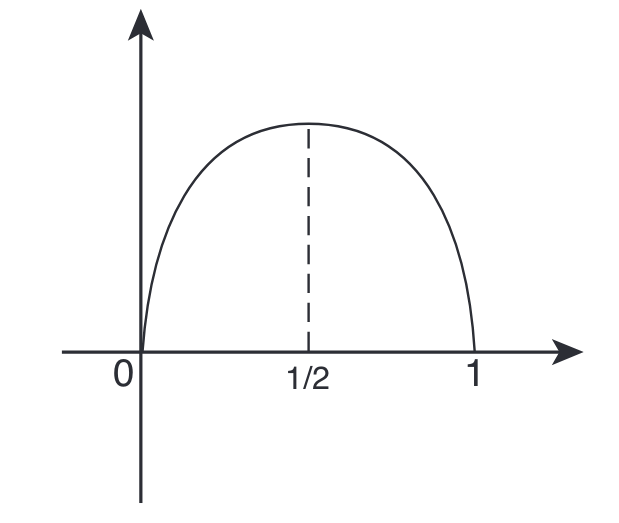
\includegraphics[scale=0.4]{graph.png}
			\caption{The graph of the binary entropy function $h(p)$.}
	\end{figure}
\end{example}

\begin{example}
	Suppose $X$ is a geometric random variable with probability $p$. Then $\Prob[X = i] = (1-p)^ip$. The entropy of $X$ is then
	\begin{align*}
		H(X) &= \sum_{i=0}^\infty (1-p)^ip\log \frac{1}{p(1-p)^i}\\
		&= \frac{h(p)}{p}.
	\end{align*}
\end{example}

\noindent Now we state a theorem about some of the nice properties entropy has. One can show that any function satisfying these properties is exactly our definition of entropy up to multiplication by a constant factor.
\begin{theorem}[Properties of Entropy]
	\begin{enumerate}
		\item $H(X)\geq 0$, with equality if and only if $H$ is constant. 
		\item $H(X) \leq \log n$ if $X$ has $n$ possible outcomes, with equality if and only if $X$ is uniformly distributed. (The most ``unpredictable'' variable is a uniform one.)
		\item $H(X) = H(f(x))$ for any bijective $f$. (The labels don't matter, only the probabilities.)
		\item $H(X|Y) \leq H(X)$, with equality if and only if $X$ and $Y$ are independent. (More information, i.e. conditioning, lowers uncertainty.)
		\item $H(X,Y) = H(X) + H(Y|X) \leq H(X)+H(Y)$. (A ``chain rule''.)
		\item $H(X) \geq H(f(X))$, with equality if and only if $f$ is injective.
		\item $H(X_1,\ldots, X_n) = \sum_{i=1}^nH(X_i|X_{j<i})$, with equality if and only if the $X_i$ are mutually independent. (A bigger ``chain rule''.)
	\end{enumerate}
\end{theorem}

\begin{proof}
	\begin{enumerate}
		\item Since $0\leq p_i\leq 1$, $-\log p_i \geq 0$, so the sum defining entropy has only nonnegative terms.
		\item The logarithm is concave, so we can apply Jensen's inequality:
		\begin{align*}
			H(X) &= \E[\log 1/p_X(x)]\\
			&\leq \log \E[1/p_X(x)]\\
			&= \log \E\left[\sum_{i=1}^n 1\right]\\
			&= \log n.
		\end{align*}
		We didn't prove it during the seminar, but a slick proof for the ``only if uniform'' part I found online uses the \href{https://en.wikipedia.org/wiki/Inequality_of_arithmetic_and_geometric_means#Weighted_AM.E2.80.93GM_inequality"}{weighted AM-GM inequality}:
		\begin{align*}
		 	2^{H(X)} &= \prod_{i=1}^np_i^{-p_i}\\
		 	&\leq \sum_{i=1}^n p_i \cdot \frac{1}{p_i}\\
		 	&= n,
		\end{align*} 
		with equality if and only if the $p_i$ are all equal.
		\item $H(X)$ depends only on the probabilities associated to the outcomes of $X$, not the outcomes themselves.
		\item We skipped the proof for this. It's allegedly coming later.
		\item Follows from the definition of the joint distribution.
		\item $x\mapsto (x, f(x))$ is injective, so by properties 3 and 5 we have
		\begin{align*}
			H(X) &= H(X, f(X))\\
			&= H(f(X)) + H(X|f(X))\\
			&\geq H(f(X)).
		\end{align*}
		We obtain equality if and only if $H(X|f(X)) = 0$, which happens if and only if $X$ is constant given $f(X)$.
		\item Same proof as property 5.
	\end{enumerate}
\end{proof}

\end{document}